\chapter{Uncertainty quantification in high dimensions}
\label{UQ}

Uncertainty quantification (UQ) endeavors to consider the uncertainties associated with the parameters in the model of a physical system and examine their influence on the system response. A well-established representation of an uncertainty quantification problem is outlined next. The premise is that any such problem can be depicted as a combination of these ingredients, as illustrated in \cref{fig: UQ_steps}:
\begin{itemize}
    \item A computational model $\mathcal{M}$. This encompasses a broad spectrum, ranging from an analytical function in its simplest form to a black box housing various levels of partial differential equations (e.g., finite element packages or finite difference packages). Generally, the computational model $\mathcal{M}$ establishes a mapping from a set of input parameters $\boldsymbol{x})$ to one or more \acrfull{QoI}, often denoted as \textit{model responses}.    
    \item The sources of uncertainties in input space. This step involves identifying the input parameters that are uncertain and describing them within a probabilistic context.
    \item Uncertainty propagation from input parameters $\boldsymbol{x}$ to $\boldsymbol{y}$. This step pertains to quantifying the \acrshort{QoI} by propagating the uncertainty of the input space through the computational model $\mathcal{M}$. 
    \item Iterative updating of the source of uncertainty. This step encompasses various techniques employed to refine the information related to the identified sources of uncertainty above. Examples includes \textit{sensitivity analysis} or \textit{Bayesian inference}. If we are using \textit{sensitivity analysis} to update the uncertainties, it can be explicitly called as \textit{forward problems}. If we are using \textit{Bayesian inference} to update the uncertainties, it can be called as \textit{inverse problems}.
\end{itemize}
\begin{figure}[htbp]
    \centering
    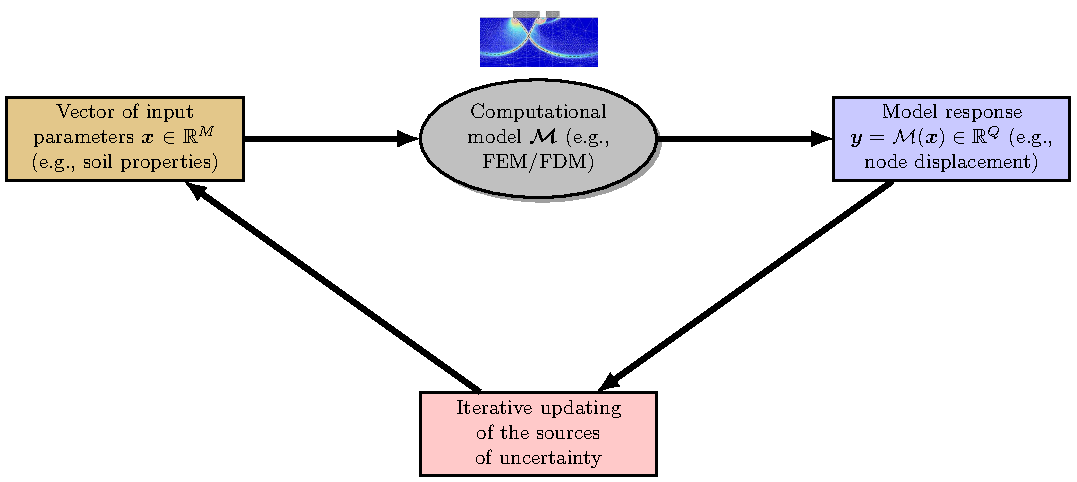
\includegraphics[width = 140mm]{Figures/figure-UQ_steps.pdf}
    \caption{Global framework for uncertainty quantification}
    \label{fig: UQ_steps}
\end{figure}


\section{Problem statement}
In modern engineering applications, uncertainty quantification (UQ) often involves simulations with a large number of input parameters. The computational model is frequently treated as a black box, where only the input parameters $\boldsymbol{x}$ and the corresponding model response $\boldsymbol{y}$ are available. Addressing uncertainties through traditional \textit{Monte Carlo} methods in such systems can be computationally intensive, posing a significant challenge. To alleviate this computational burden, surrogate models $\tilde{\mathcal{M}}$, illustrated in \cref{fig: UQ_surrogate}, can be employed. The solid line denotes the current working flow. These surrogate models approximate the original model with a cost-effective replacement model, allowing for efficient exploration of the input parameter space. A surrogate model $\tilde{\mathcal{M}}$ can be then expressed as:
\begin{equation}
\label{eq:surrogate_model}
    \tilde{\mathcal{M}}(\boldsymbol{X})  \overset{\mathrm{def}}{=} \mathcal{M}(\boldsymbol{X}) - \mathcal{R}(\boldsymbol{X})
\end{equation}
where $\mathcal{R}$ is the residual between the original model and the surrogate. The overarching concept of \cref{eq:surrogate_model} is straightforward: working with a finite set of input parameters and their corresponding model outputs, commonly referred to as an \textit{experiment of design}.
\begin{figure}[htbp]
    \centering
    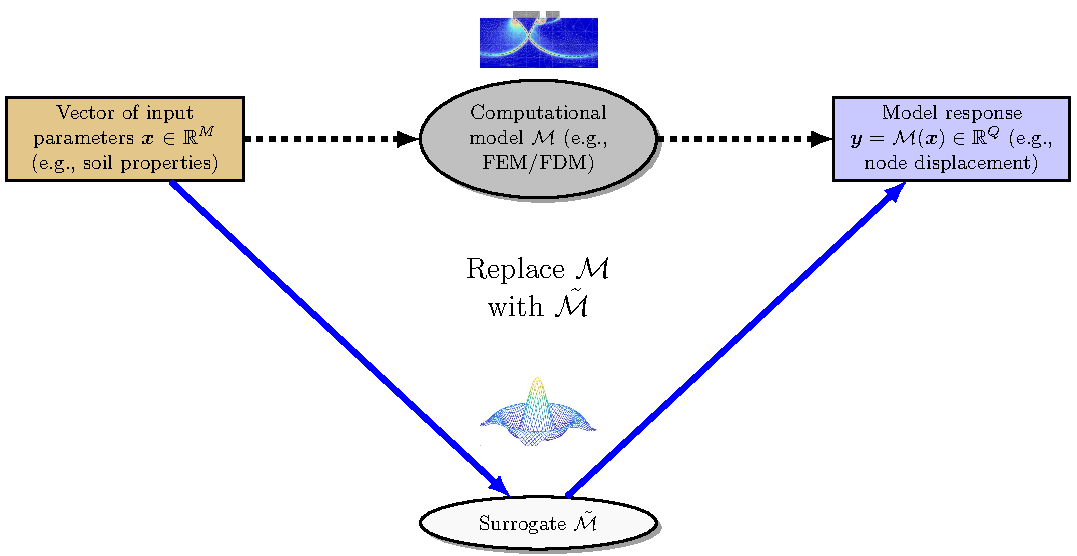
\includegraphics[width = 140mm]{Figures/figure-UQ_surrogate.pdf}
    \caption{Using a surrogate to obtain the model response}
    \label{fig: UQ_surrogate}
\end{figure}

 In high dimensions scenarios, surrogate models tend to exhibit diminished performance, coupled with escalating computational and storage costs-a challenge commonly acknowledged as the \textit{curse of dimensionality}. Consequently, challenges may arise from: 
 
 (1) in large-scale scenarios, the computational intractability of conducting thousands of forward simulations is a common challenge; (2) the complexity of the input/output space dimensions adds another layer of difficulty;(3) the large dimensionality of the input/output space complicates the sampling process;
 Thus, to alleviate this in a statistical inverse problems, methods can be broadly categorized in three groups: (1) choose an appropriate type of surrogates to accelerate a forward simulation; (2) reduce the size of the input/output space, i.e., sensitive analysis or \acrlong{DR} techniques; (3) sequential efficient sampling method in \textit{experiment of design} (\textit{active learning}) or in a posterior (e.g., \acrshort{MCMC}).


\section{Surrogate model choices}
 

\begin{table}[htbp]
\caption{Surrogate model choices}
\label{table: All_Surrogates}
\begin{tabular}{lll}
\hline
Name                              & \multicolumn{1}{c}{Shape} & \multicolumn{1}{c}{Parameters} \\ \hline
Polynomial chaos expansions       &                           $\tilde{\mathcal{M}}(\boldsymbol{x})
=
\sum_{\boldsymbol{\alpha} \in \mathcal{A} } 
\boldsymbol{y_{\alpha}} \Psi_{\boldsymbol{\alpha}} (\boldsymbol{x})$&                                $\boldsymbol{y_{\alpha}}$\\
Low-rank tensor approximations    &                           $\tilde{\mathcal{M}}(\boldsymbol{x})
=
\sum_{l=1}^{R} b_{l}
\left ( 
\prod_{i=1}^{M}  v_{l}^{i}x_{i}
 \right ) 
$&                                $b_{l}, \  z_{k,l}^{i}$\\
Kriging (a.k.a Gaussian processs) &                           $\tilde{\mathcal{M}}(\boldsymbol{x})
=
\boldsymbol{\beta}^{T} \cdot \boldsymbol{f}(\boldsymbol{x})
 + Z(\boldsymbol{x},\omega)$&                                $\boldsymbol{\beta}, \ \sigma_{Z}^{2}, \  \boldsymbol{\theta}$\\
Support vector machines           &                           $\tilde{\mathcal{M}}(\boldsymbol{x})
=
\sum_{i=1}^{m}
a_{i} K(\boldsymbol{x}_{i},\boldsymbol{x}) 
+b$&                                $\boldsymbol{a}, \ b$\\
Neural networks                   &                           $\tilde{\mathcal{M}}(\boldsymbol{x})
=
f_{n}\left ( 
\cdots f_{2}(
b_{2} + f_{1}(
b_{1} + \boldsymbol{w}_{1} \cdot \boldsymbol{x}
)
\cdot \boldsymbol{w}_{2}
)
\right ) $&                                $\boldsymbol{w}, \ \boldsymbol{b}$\\ \hline
\end{tabular}
\end{table}
Ongoing research on surrogate modelling focuses on various problems, like hyperparametes tuning, mathematical explanation or the accuracy based on few observations. A range of techniques exist in surrogate modelling, in which some of them are listed in the \cref{table: All_Surrogates}. Among these popular surrogate models above, it is crucial to choose the most appropriate model for our own geotechnical problem. Inspired by \cite{torre2019}, we only focus on \acrfull{PCE} which is presented next. Compared with other surrogate models based on benchmark data sets (e.g., \textit{Ishigami function}, \textit{23-bar horizontal truss}), \acrshort{PCE} exhibits additional advantageous properties, such as:
\begin{itemize}[left=0pt]
    \item \acrshort{PCE} excels in various tasks, necessitating only minimal parameters tuning for adaptation to specified data considerations.
    \item \acrshort{PCE} not only provides precise point-wise predictions for the output at given inputs, but also furnishes relevant statistics in the presence of input uncertainties. This benefits in UQ process as it results from the integration of the \acrshort{PCE} model with a suitable probabilistic characterisation of the input model.
    \item The coefficients of \acrshort{PCE} makes it free to get sensitivity analysis results.
    \item The output produced by \acrshort{PCE} is analytically expressed as a simple polynomial of the input. This characteristic makes the model easy to interpret from a mathematical standpoint. This is in contrast with black-box models (e.g., neural networks) or classification-based models (e.g., tree models), where our reliance is placed on the assumption that training data is sufficiently big to yield an accurate surrogate.
    \item \acrshort{PCE} achieves acceptable performance levels with a relatively 
    modest amount of data in the \textit{experiment of design}.
\end{itemize}
Note: The choice for \acrshort{PCE} in our thesis does not guarantee the conclusion that \acrshort{PCE} outperforms than other surrogate models. The properties obtained above are only based on some simple toy problems. Therefore, a choice for surrogate models is problem-specified and it is not always the same case when it encounters into different geotechnical problems. However, the \acrshort{PCE} advantages above \citep{torre2019} indeed give us confidence to get started with \acrshort{PCE} first. But other advanced surrogate models can be also easily employed.


\section{Polynomial chaos expansion}
Polynomial chaos expansions (PCE) represent a potent metamodelling technique designed to provide a functional approximation of a computational model. This approximation is achieved through its spectral representation of the model on a carefully built basis of polynomial functions. Consider a random vector with independent components $\boldsymbol{X} \in \mathbb{R}^{M}$ characterized by the joint \acrshort{PDF} $f_{\boldsymbol{X}}$. Additionally, suppose there exists a computation model with finite variance, defined as a mapping $Y = \mathcal{M}(\boldsymbol{X})$, with $Y \in \mathbb{R}$. This can be expressed as follows:
\begin{equation}
    \mathbb{E}[Y^2] 
    =\int_{\mathcal{D}_{\boldsymbol{X}}}
    \mathcal{M}^2(\boldsymbol{x})f_{\boldsymbol{X}}(\boldsymbol{x})
    d\boldsymbol{x}< \infty 
\end{equation}
Then, a \acrshort{PCE} $\mathcal{M}(\boldsymbol{X})$ can be represented as:
\begin{equation}
\label{eq: PCE_basis}
Y=\mathcal{M}(\boldsymbol{X}) \approx
\sum\limits_{\alpha \in \mathcal{A} }{\boldsymbol{y_{\alpha}} \Psi_{\boldsymbol{\alpha}}(\boldsymbol{X})}
\end{equation}
where $\Psi_{\boldsymbol{\alpha}}(\boldsymbol{X})$ denotes multivariate polynomials orthonormal relative to $f_{\boldsymbol{X}}$, The multi-index $\boldsymbol{\alpha} \in \mathcal{A}$ identifies the truncated multivariate polynomials $\Psi_{\boldsymbol{\alpha}}$. $\boldsymbol{y_{\alpha}} \in \mathbb{R}$ corresponds to the corresponding coefficients. There are four main ingredients for a \acrshort{PCE}: (1) Construct the basis functions $\Psi_{\boldsymbol{\alpha}}$; (2) Compute the coefficients $\boldsymbol{y_{\alpha}}$; (3) Evaluate the precision of the \acrshort{PCE}; (4) Post process the \acrshort{PCE}. A visualized \acrshort{PCE} example with a two-dimensional input can be seen in \cref{fig: PCE_visual}.
\begin{figure}[htbp]
    \centering
    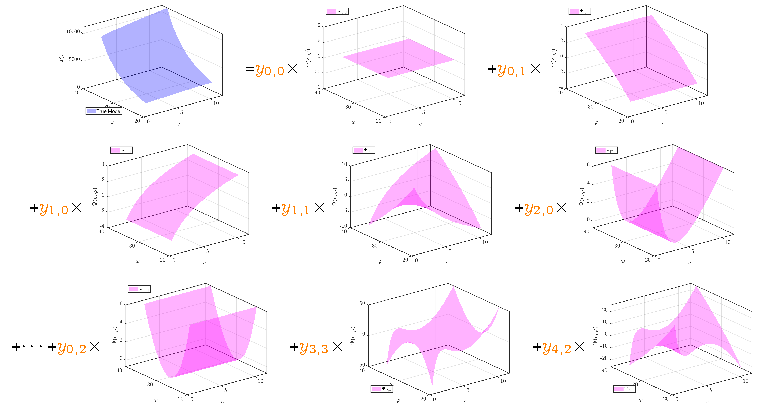
\includegraphics[width = 140mm]{Figures/figure-PCE_visualize.pdf}
    \caption{PCE visualization in a two-dimensional example from \protect\cite{PCE-visual}}
    \label{fig: PCE_visual}
\end{figure}



\subsection{Construct the basis functions $\Psi_{\alpha}$}
The polynomial basis $\Psi_{\boldsymbol{\alpha}}(\boldsymbol{x})$ in \cref{eq: PCE_basis} is conventionally constructed using a set of \textit{univariate orthonormal polynomials} $\phi_{k}^{i}(x_{i})$, where these polynomials satisfy:
\begin{equation}
    \left \langle 
\phi_{j}^{i},\phi_{k}^{i}
 \right \rangle 
= \delta_{jk}
\end{equation}
$\delta_{jk}$ is the \textit{Kronecker symbol}. The multivariate polynomials $\Psi_{\alpha}$ are then constructed by taking the tensor product of their univariate counterparts:
\begin{equation}
\Psi_{\boldsymbol{\alpha}}(\boldsymbol{x})
 \overset{\mathrm{def}}{=}
\prod_{i=1}^{M} 
\phi_{\alpha_{i}}^{i}(x_{i})
\end{equation}
in which, $\boldsymbol{\alpha}= \{\alpha_{1},\cdots,\alpha_{M}\}  \ \alpha_{i} \in \mathbb{N}^{M}$ of degree $|\boldsymbol{\alpha }|=\sum_{i=1}^{M} \alpha_{i}$, and $\Psi_{\boldsymbol{\alpha}}(\boldsymbol{x})$ satisfies orthonormal properties as:
$        \left \langle 
\Psi_{\boldsymbol{\alpha}}(\boldsymbol{x}),\Psi_{\boldsymbol{\beta}}(\boldsymbol{x})
 \right \rangle 
= \delta_{\boldsymbol{\alpha}\boldsymbol{\beta}}$, where the symbol $\delta_{\boldsymbol{\alpha}\boldsymbol{\beta}}$ is an extension \textit{Kronecker symbol} to the multi-dimensional case. Classical families of orthogonal polynomials have been discovered historically in \cref{table: Polynomial_family}. 
\begin{table}[]
\caption{Univariate orthogonal polynomials}
\label{table: Polynomial_family}
\centering
\begin{tabular}{lll}
\hline
\textbf{Name}& \textbf{Support $\mathcal{D}_{\boldsymbol{X}}$}& \textbf{Weight function $f_{\boldsymbol{X}}$}\\ \hline
Legendre&            $[a;b]$&                    uniform\\
Jacobi&            $[a;b]$&                    Beta\\
Hermite&            ($-\infty;\infty$)&                    Gaussian\\
Laguerre&            $[;\infty)$&                    Gamma\\ \hline
\end{tabular}
\end{table}
\begin{equation}
A^{M,p,q} = \{\alpha \in A^{M,p} : ||\alpha||_q \leq p\}; \ {\rm{where}}  \   
||\alpha||_q = \left(\sum_{i=1}^{M} \alpha_i^q\right)^{1/q}
\end{equation}
The infinite series expansion cannot be handled in practical computations. Two truncation schemes can be applied: (1) restriction of maximum interaction $p$; (2) reduce hyperbolic truncation $q$. An example of the truncation in two dimensions for various values of $p$ and $q$ is depicted in \cref{fig: PCE_truncation}.
\begin{figure}[htbp]
    \centering
    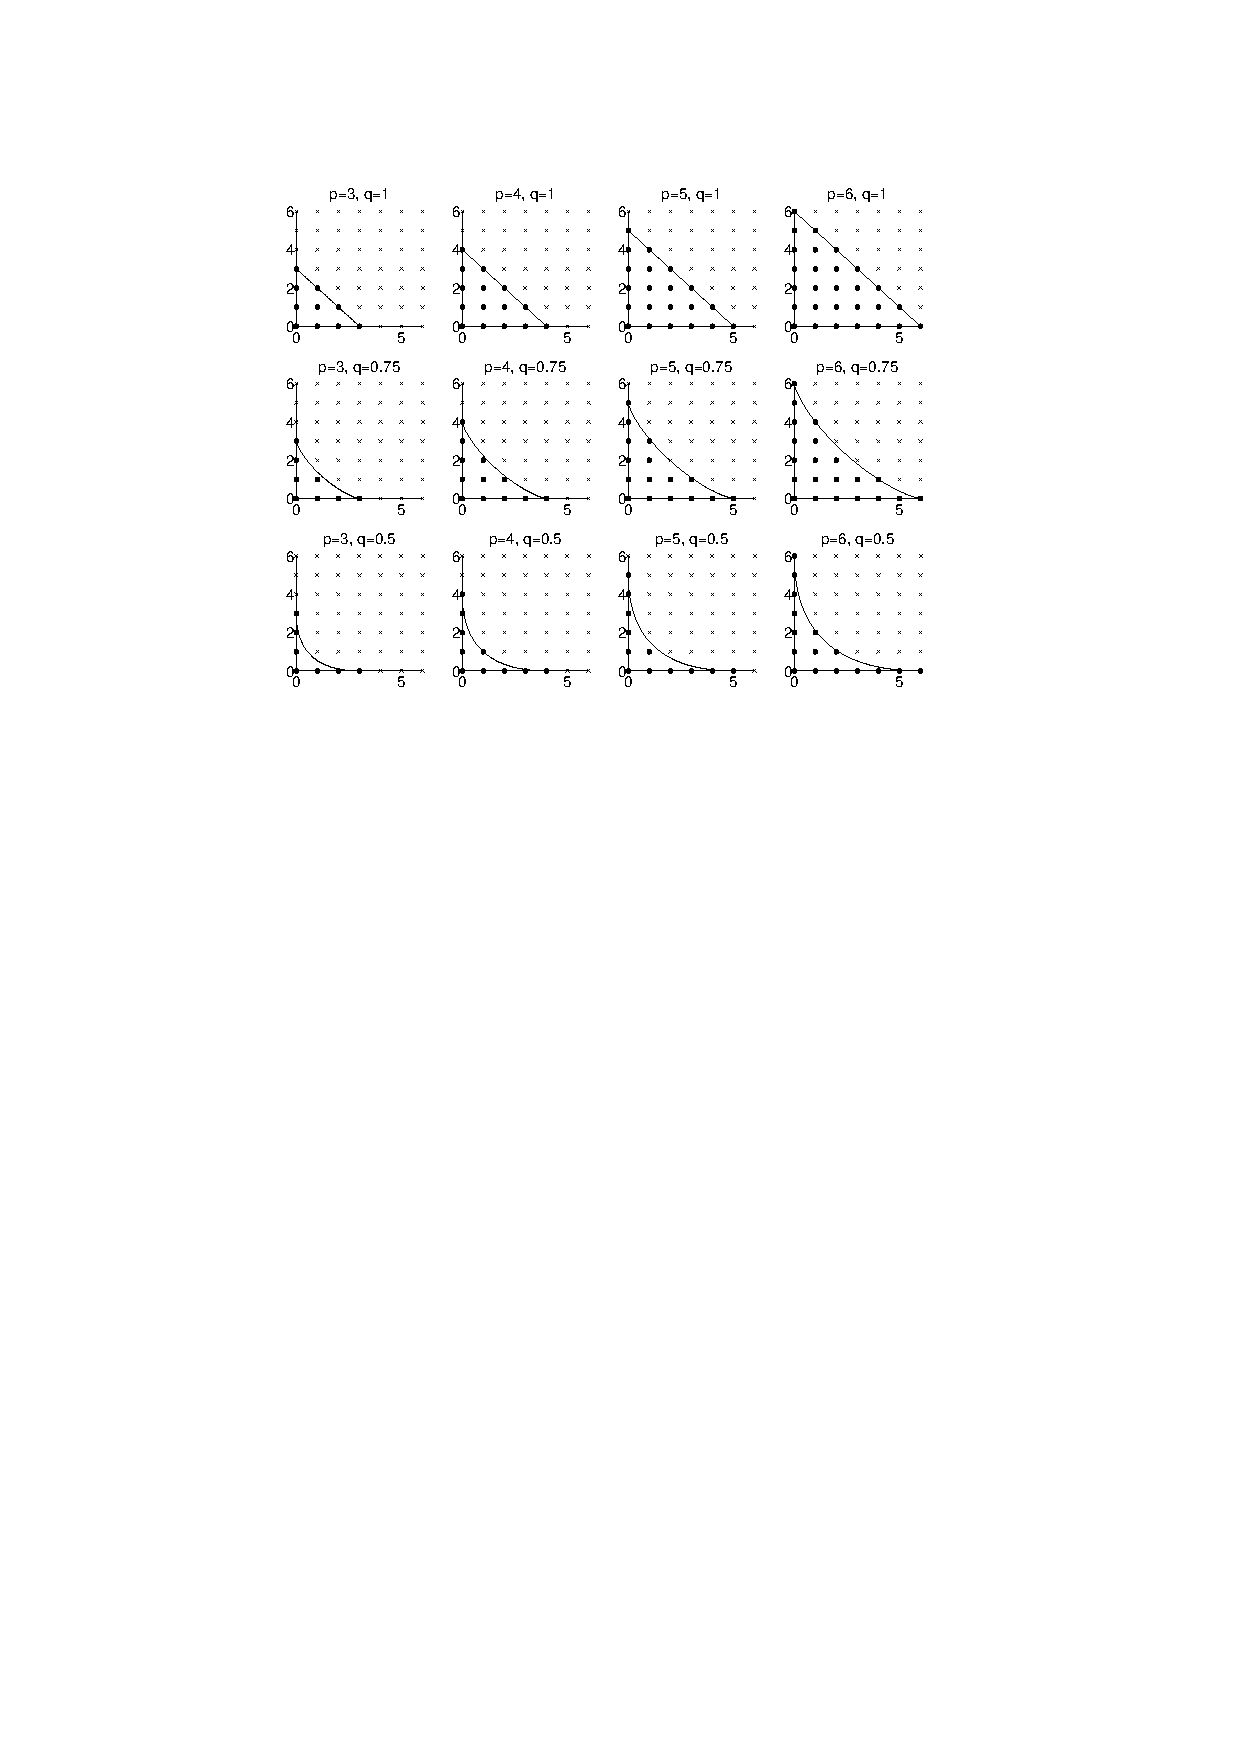
\includegraphics[width = 140mm]{Figures/figure-PCE_truncation.pdf}
    \caption{Truncation set for varying values of $p$ and $q$ from \cite{UQdoc}}
    \label{fig: PCE_truncation}
\end{figure}


\subsection{Compute the coefficients $y_{\alpha}$}
Various methods are available for computing the coefficients $\boldsymbol{y_{\alpha}}$ of the \acrshort{PCE} with a known basis. Two primary strategies commonly employed are \textit{projection} and \textit{regression}. \textit{Projection} methods leverage the orthogonality of the basis to determine the coefficients. On the other hand, \textit{regression} methods utilize standard linear regression approaches to solve the system. Below are some of the methods:

\subsubsection{Projection method}
The evaluation of the polynomial coefficients $\boldsymbol{y_{\alpha}}$ can be reformulated as the calculation of the expectation value in 
\begin{equation}
\label{eq: PCE_projection}
\boldsymbol{y_{\alpha}} = E [\Psi_{\boldsymbol{\alpha}}(\boldsymbol{X}) \cdot \mathcal{M}(\boldsymbol{X})]
\end{equation}

\subsubsection{Least-squares minimization}
This approach casts \cref{eq: PCE_projection} as a least-squares minimisation problem as shown:
\begin{equation}
\boldsymbol{\hat{y}_{\alpha}} = {\rm{argmin}} \mathbb{E} [\varepsilon_{P}^2(\boldsymbol{X})] = {\rm{argmin}} \mathbb{E} [(\tilde{\mathcal{M}}(\boldsymbol{X}) - \mathcal{M}(\boldsymbol{X}))^2]
\end{equation}
Some other regression methods can be also easily implemented, i.e., \textit{ordinary least square}, \textit{compressive sensing} or \textit{stochastic collocation}.


\subsection{Check the accuracy of the \acrshort{PCE}}
Error estimators are essential for quantifying the fidelity of a surrogate model in approximating the original model. To determine the precision of a surrogate, \textit{leve-one-out} (LOO) is a good way to assess the cross validation error. For a \acrshort{PCE} consisting $N$ metamodels, error $\varepsilon_{\text{LOO}}$ can be shown as:
\begin{equation}
\varepsilon_{\text{LOO}} = \frac{1}{N} \sum_{i=1}^{N} \left( \mathcal{M}(\boldsymbol{x}^{(i)}) - \tilde{\mathcal{M}}(\boldsymbol{x}^{(i)}) \right)^2
\end{equation}




\subsection{Post process the \acrshort{PCE}}
Due to the inherent orthogonality with the polynomial basis functions, we can derive explicit expressions for moments characterizing the model output. The first pair moments of a \acrshort{PCE} find their manifestation within is coefficients. Specifically, the mean and variance of a \acrshort{PCE} manifest as:
\begin{equation}
E[Y] = \mathbb{E}[\tilde{\mathcal{M}}(\boldsymbol{X})] = y_{\boldsymbol{0}}
\end{equation}
\begin{equation}
\text{Var}[Y] = E[Y^2] - E[Y]^2  \approx \sum_{\alpha \in A \setminus \{0\}} y_{\alpha}^2
\end{equation}
Another crucial aspect of \acrshort{PCE} post-processing lies in the fact the coefficients encapsulate significant details regarding the \textit{ANOVA} decomposition of a surrogate. This information can be harnessed to efficiently compute global sensitivity at a minimal computational expense. Because it is popular to make choices on the most important variables and update the uncertainties based on the sensitivity results. Thus, strictly speaking, \textit{sensitivity analysis} also belongs to the category of \acrshort{DR}. 

\section{Dimensionality reduction}


Geotechnical problems inherently involve high dimensionality, posing challenges for learning methods like surrogate modeling. Technical constraints impact the storage and processing of such huge amount of data. Furthermore, as input and output data expand, independent scalar surrogate models show inadequate in accurately capturing the covariance matrix of the original data, leading to less reliable predictions. Consequently, in high dimensional space, the need for \acrfull{DR} becomes more critical. 

The transformation from the \textit{original space} $\mathcal{D}_{\boldsymbol{Y}} \subseteq \mathbb{R}^{N}$ to a \textit{reduced space} $\mathcal{D}_{\boldsymbol{Z}} \subseteq \mathbb{R}^{n}$ with $n \ll N$ is the general form of a \acrshort{DR} mapping:
\begin{equation}
    \mathcal{T}_{DR} : \mathcal{D}_{\boldsymbol{Y}} \rightarrow \mathcal{D}_{\boldsymbol{Z}}
\end{equation}
where the underlying assumption is that $\mathcal{D}_{\boldsymbol{Z}}$ is embedded inside $\mathcal{D}_{\boldsymbol{Y}}$. There exists a large set of \acrshort{DR} techniques ranging from linear to nonlinear approaches. A simple but effective linear technique, that is widely used today, is the \textit{principal component analysis} (\acrshort{PCA}). It is popular across a wide range of disciplines and is closely related to the \textit{Karhunen-Loève expansion} and \textit{proper orthogonal decomposition}. In practical applications, the \acrshort{PCA} process is involves the estimation of the expectation $\boldsymbol{\mu_{Y}} \approx \mathbb{E}[\boldsymbol{Y}]$ and the covariance matrix $\Sigma_{\boldsymbol{Y}} \approx Cov[\boldsymbol{Y}]$. The $N$ eigenvectors of this covariance matrix are represented by $\phi_{p}$ for $p=1,\cdots,N$. The corresponding eigenvalue $\lambda_{p}$ signifies the variance of $\boldsymbol{Y}$ in direction of the $p-th$ principle component. Consequently, the random vector $\boldsymbol{Y}$ can be expressed through its $n$ principal components with the highest variance:
\begin{equation}
\boldsymbol{Y} \approx \boldsymbol{Y}^{PCA} 
= \boldsymbol{\mu_{Y}} + 
\sum_{p=1}^{n} z_{p}\phi_{p}
\end{equation}
The selection of the number $n$ is determined such that $\sum_{p=1}^{n} \lambda_{p} = 
(1-\varepsilon_{0})\sum_{p=1}^{N} \lambda_{p}$, where $\varepsilon_{0}$ typically set to 0.01. Consequently, the model output $\boldsymbol{Y} \in \mathbb{R}^{N}$ can be processed by a linear transformation of the principle component vector $\boldsymbol{Z} = (z_{1},\cdots,z_{n})$. This reduction in the dimensionality, from $N$ to $n$ $n \ll N$, is then achieved. When data sets become more complex, more advanced \acrshort{DR} techniques can be used, such as \textit{multi-dimensional scaling}, \textit{kernel principal component analysis} and \textit{auto-encoder}.


\section{DR-based surrogate in Bayesian inference}
In high dimensions, a popular two-step approach is frequently adopted to address such challenges: first, the input/output dimensions are reduced; subsequently, the surrogate model is directly constructed within the \textit{reduced space}. Performance of DR-based surrogate has showed superior performance in some benchmarks \citep{lataniotis2019}. Take \acrshort{PCA} and \acrshort{PCE} as a \acrshort{DR} example in \cref{fig: PCA-PCE}, the amalgamation of \acrshort{PCA}-\acrshort{PCE} constitutes an efficient surrogate modelling technique. The solid line denotes the current working flow. 

\begin{figure}[htbp]
    \centering
    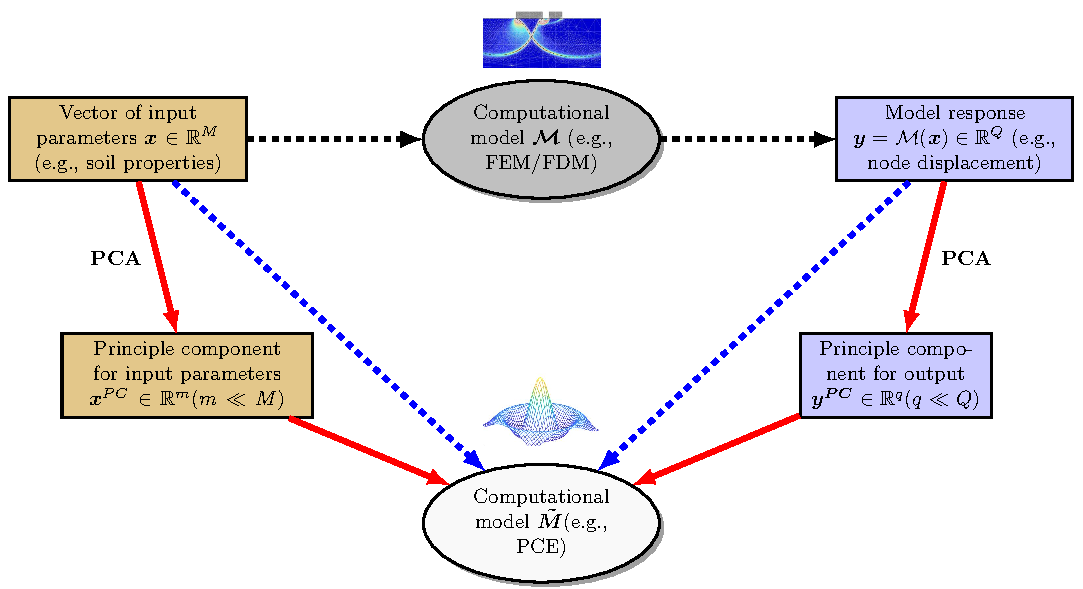
\includegraphics[width = 140mm]{Figures/figure-PCA_PCE.pdf}
    \caption{\acrfull{DR} schematic example}
    \label{fig: PCA-PCE}
\end{figure}
When it comes to Bayesian inference process accelerated by DR-based surrogate, working principles can be shown in \cref{fig: PCA-PCE-BI} as below:
\begin{itemize}[left = 0pt]
    \item Step one: \acrshort{PCA} technique reduces the size of input/output into principal components.
    \item Step two: construct \acrshort{PCE} based on the principal components from step one.
    \item Step three: Pass obtained \acrshort{PCE} into Bayesian inference process and evaluate the likelihood. 
\end{itemize}
\begin{figure}[H]
    \centering
    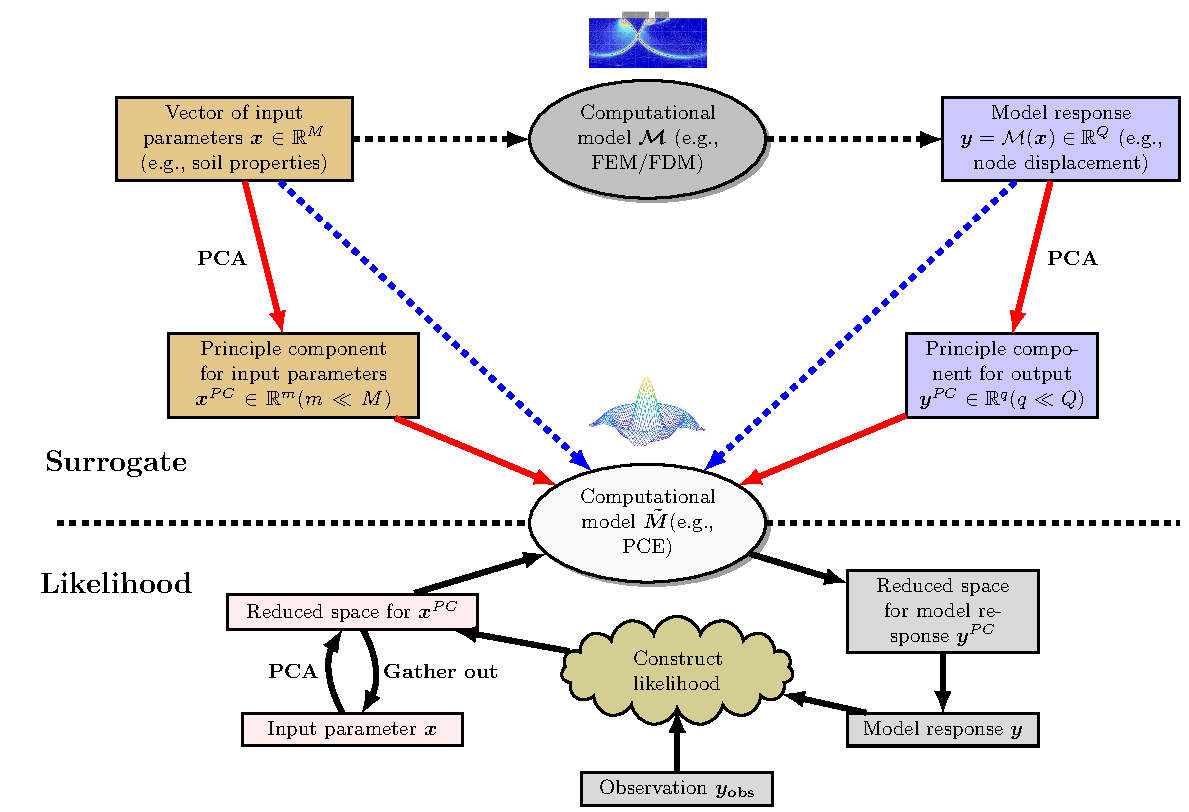
\includegraphics[width = 140mm]{Figures/figure-PCA_PCE_BI.pdf}
    \caption{Bayesian inference accelerated by a PCA-PCE surrogate}
    \label{fig: PCA-PCE-BI}
\end{figure}
Note: DR-based surrogates are not only limited to Bayesian inference in high dimensions. Even in low dimension's inference, DR-based surrogates still outperform than the case with surrogate models without any \acrshort{DR}. Because \acrshort{DR} is more than a data compressing technique in Bayesian inference, it can capture the covariance matrix of the original data to make more accurate predictions. Due to this feature, compared to the traditional scalar models (e.g., PCE, kriging), DR-based surrogates make it possible to consider multiple outputs predictions.





